\chapter{Megértés}

\keywords{tények és tapasztalat, kétség, tények halmozása}

\noindent Részekre osztjuk az ismeretet és fokozatos lépésekben
beszélünk a gyakorlásról, de a megértés egyszerre történik. Az
észrevétel azonnal történik -- az `Aha!' pillanat, amikor eloszlik a
köd. Kezdetben szükséges némi információ, de emlékszünk arra, hogy a
tanítás igazságát mindenki a saját tapasztalatán keresztül éli meg. A
meditáció gyakorlásában azok a tények hasznosak számunkra, amik
\emph{itt-és-most} tények, amit a jelen pillanatban megismerünk.

Ha csupán külső információra támaszkodunk, vagy folyton egy újabb
élményre várunk, sosem érkezünk meg oda, ahol megállhatunk. Ez a
függőség kimerítő. Egyre több kétséget és mentális nyugtalanságot hoz
létre. Hiába halmozunk fel egyre több tényt, egyre keserűbben érezzük
magunkat, és erősödik a belső hiányérzet. Nem több információra van
szükségünk, hanem ennek a szükségnek az elengedésére. Akkor tudunk
nyugodtan megállni.

\keywords{érzéki tapasztalat, azonosulás}

Az emlékek, érzékelés és elvárások egy tapintható erővel húznak-tolnak
minket. Míg az élmények maguk eltűnnek, a kényszer sosem pihen: máris a
következőt akarjuk. Hogyan lehetnek ezek a jelenségek olyan meggyőzőek,
hogy folyton húznak minket előre? Az táplálja a folyamatot, hogy
\emph{magunkat látjuk bennük.} Úgy látjuk, hogy ezek vagyunk, ezek
voltunk, ezek leszünk, és mivel szüntelenül változnak és felbomlanak,
egyre tovább folytatjuk, várjuk a következőt.

\clearpage
\figurepagelayout

\begin{figure}[h]
\vspace*{-15pt}
\caption{Érzet és Azonosulás}\label{fig-feeling-identification}
\bigskip
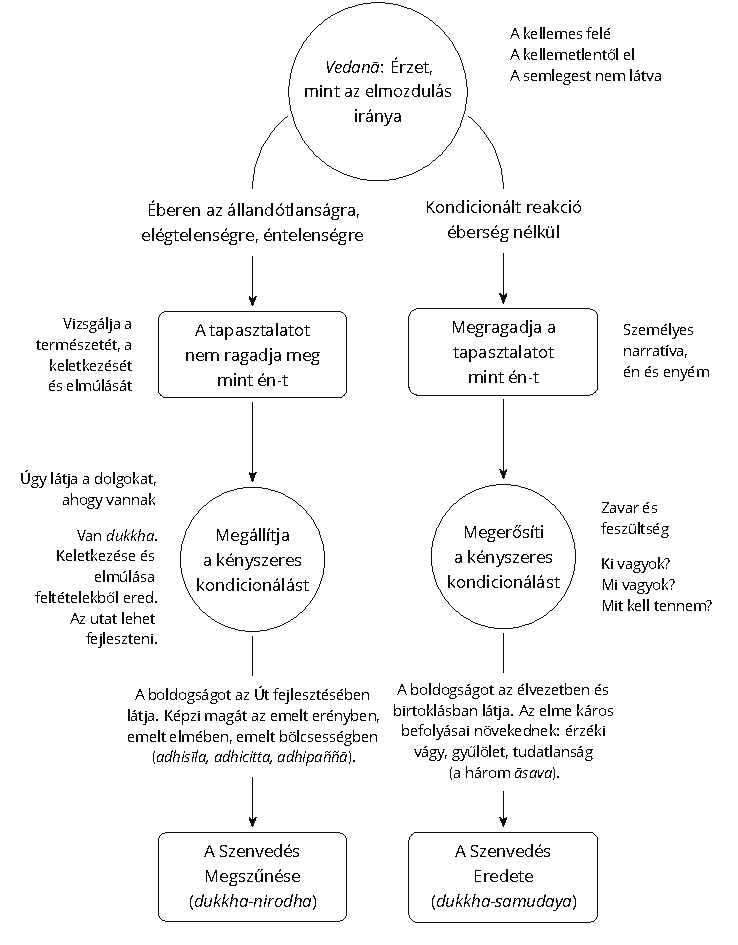
\includegraphics[width=\linewidth]{./manuscript/tex/diagrams/feeling-identification-hu.pdf}
\vspace*{\baselineskip}
\end{figure}

\clearpage
\normalpagelayout

Mi lenne, ha egy nap úgy ébrednénk fel, hogy semmire sem emlékszünk a
múltból? A tapasztalatunkat ilyen állapotban is megragadnánk, mint
\emph{én és enyém}. Annyira kiborító lehetne, hogy félelemtől bénulva
feküdnénk amíg meg nem tudunk ragadni valamilyen történetet, ami
megmagyarázza hol és kik vagyunk. Nem is kell elveszíteni a memóriánkat,
hogy ezt megfigyeljük: utazás közben lekésni egy fontos csatlakozást is
elég ijesztő lehet, hogy így érezzük magunkat, vagy más alkalommal
amikor nem tudjuk a helyzetünket irányítani.

Alázatra késztet mikor észrevesszük, mennyi mindent személyes ügynek
tekintünk, pedig észszerűen gondolkodva tudjuk, hogy nem kellene. A
Buddha azt tanítja, hogy az elme továbbra is az `én és enyém' képzetét
alkotja az érzékek tapasztalatából, amíg ennek a tapasztalatnak a
mulandóságát nem értjük teljesen. Személyes ügynek tekintjük és meg
vagyunk győződve, hogy vagy (1) `Ez én vagyok', (2) `Én ebben vagyok',
(3) `Én ezen kívül vagyok', (4) `Ez az enyém', vagy (5) `Én örömöt
találok ebben'.\footnote{\href{https://a-buddha-ujja.hu/mn-1/hu/pressing-lajos}{MN
  1}, A létesülés gyökeréről szóló tanítóbeszéd}

Jaj, szegény elménk, miért nem vagyunk bölcsebbek? Kezdhetjük azzal,
hogy kevés figyelmünk jut másra, miközben szokás szerint azzal vagyunk
elfoglalva, hogy arról gondolkodunk hogyan kapjuk meg amit akarunk, és
arról panaszkodunk, amit nem kaptunk meg.

Mikor az érzék-kapu kontaktusba kerül egy érzék-tárggyal, ha jelen van a
figyelem, a tapasztalatot a három érzés (\emph{vedanā}) közül egyikként
érezzük, amit hasonlíthatunk ahhoz, hogy milyen irányba mozdulunk:

A kellemes felé, el a kellemetlentől, vagy békében maradunk a
semlegessel. A képzetlen elme gépiesen követi ezeket a megalapozott
mintákat és a mögöttesen húzódó hajlamok magukkal sodorják: a
szenvedély, gyűlölet és tudatlanság.

Ebben a tekintetben, az ember akkor érti az érzéseket, amikor érti az
érzékek kontaktusát. Ennek eredménye, hogy az ember a kellemeset
fájdalmasnak látja (mivel végső soron elégtelen a természete), a
fájdalmasat tüskeként látja (amit el kell távolítani, vagy türelemmel
elviselni), és a semlegeset állandótlannak látja (nem ringatja magát
tudatlanságba).

Ez magában foglalja, hogy nem gondol rájuk úgy, mint `én és enyém'.
Megismerjük őket, de a tudás nem lesz a \emph{miénk}. Nem tartoznak egy
személyhez, \emph{akié} az érzés.

\begin{quote}
Teljesen megértve az érzéseket,\\
Megtisztul még ebben az életben.\\
A Tanban szilárdan áll: a test széthullásakor,\\
A tudás mesterét sehol sem találni.

\bigskip

\quoteRef{%

\href{https://suttacentral.net/sn36.5/en/bodhi}{SN 36.5}, Látni kell

}
\end{quote}

\keywords{gondolkodás, leterhelve, érzekek visszafogása}

Sokat gondolkodhatunk erről, de ha analitikusan próbáljuk megérteni,
csak a fejünk fog megfájdulni. Ezt a megértést a testen keresztül kell
fejleszteni: egy jó kezdőpont az érzékek visszafogásának gyakorlása.

Figyelmesen őrizzük az érzék-kapukat. A tiszta éberség megtart egy
teret, egy kis távolságot a tudatosságunk és annak tartama között.
Amikor egy formát látunk, hangot hallunk, stb., nem ragadjuk meg a
tapasztalatot, sem mint ahogy egészben látjuk, sem egy-egy adott
jellemzőjét amit kedvelünk vagy nem. Lehet, hogy kedveljük a
tapasztalatot, de nem válunk tőle mámorossá. Lehet, hogy visszataszító a
tapasztalat, de nem húzzuk fel magunkat és nem válunk haragossá tőle.
Figyelmünk egy részét a lélegzeten tarthatjuk, vagy fenntarthatunk egy
tágas tudatosságot a test egészére -- ez segít támpontot találni, egy
biztos alapot, ami a bölcsesség készségünket informálja. Ha nem a
lélegzetre figyelünk, az is jól beválik, ha a pillanatnyi tevékenységünk
egy aspektusát figyeljük, mint amilyen a toll érintése írás közben, a
talpunkon érzett nyomás a padlón, vagy a test más érzetei.

Ez a testen alapuló gyakorlat egyszerűbb, mint intellektuális
megközelítés. Összegyűjti a mentális erőnket, és egy természetes
ritmusnak megfelelően, vagy csendes nyugalom, vagy figyelmes vizsgálódás
követi.

Észrevesszük, hogy képesek vagyunk megállni, és ami most velünk van, az
is elegendő. Gondolj arra, mit használtál a mai nap, tárgyakra és
információra is tekintettel? Lehet, hogy sok dolog van a tulajdonodban, de
egy napra egy kevés is elég. Nincs szükségünk annyi mindenre mint ahogy
gondoljuk, és lemondani róla nem veszteség, hanem egy teher alóli
felszabadulás. Ebben a visszafogottságban erőt és energiát találunk,
amit korábban a szétszórt vágy emésztett fel. A visszafogottság mindig
kéznél van, és nem veszélyeztetik külső tényezők.

Olyan ez, mikor megtanulsz kevesebbet pakolni a hátizsákodba egy túra
előtt. Némi tapasztalat után, nem is érted, miért kellett annyi mindent
cipelned korábban. Az erény olyan tettekből áll, amik boldogsághoz
vezetnek, és az erényt önmagunk felé is fordíthatjuk: a lemondás éppen
egy ilyen személyes erény. A megértés információval látja el az erényt,
és a boldogság, ami ebből születik, ebbe a megértésbe vetett bizalmat
erősíti.

\keywords{ānāpānasati, érzékek kontaktusa, érzetek, érzés}

A légzést figyeljük, és az érzékek működését. A szem formákat lát, és
megjelenik egy érzet. A fül hangokat hall, a test szilárdságot, hideget
és meleget érzékel. Ha van kontaktus az érzék-kapu és érzék-tárgy
között, megjelenik az érzet. A folyamat nem rajtunk múlik, ha van
kontaktus, nem választhatjuk, hogy ne jelenjen meg az érzet. Amikor a
kontaktus az érzék-kapu és érzék-tárgy között megszakad, megszűnik az
érzet. A jelenség a kontaktustól függően keletkezik és múlik el -- ebből
állt a tapasztalatunk. A mozdulatainkat irányíthatjuk, de ezen túl a
tapasztalat folyamatába nincs beleszólásunk: nem rólunk szól.

Amikor ezt nem vesszük észre, úgy gondoljuk a miénk az érzés. Ha az
érzettel jó érzés jár, azt várjuk nyerni fogunk belőle valamit, és ezért
ragaszkodunk hozzá. Az ilyen helytelen megértés húzódik a szükség és
nyugtalanság érzése mögött. Amikor csalódunk az elvárásainkban,
hajlamosak vagyunk feltenni, hogy mi rontottuk el valahogy, vagy valaki
más hibája volt. Egy másik élményt kezdünk keresni, ami majd megfelelőbb
lesz, és azt reméljük ez az új élmény nem így fog lejátszódni.

\enlargethispage*{2\baselineskip}

Az érzékek kapcsolatát így figyelve, az érzések már nem vonzóak vagy
visszataszítóak. Látjuk, hogy egyik hajlam sem lesz stabil és
megbízható. Ez nem tompaság. A meditációban a tapasztalat felé
fordulunk, nem attól el. Ehelyett egy érzékeny, higgadt figyelmet
fejlesztünk. Éberek és érzékenyek maradunk a tapasztalatra, de az már
nem irányít, és nem kavar fel minket. Nyugodtak maradunk.

\clearpage
\figurepagelayout

\begin{figure}[h]
\caption{Érzék-Kapcsolat és Érzet}\label{fig-sense-contact-feeling}
\bigskip
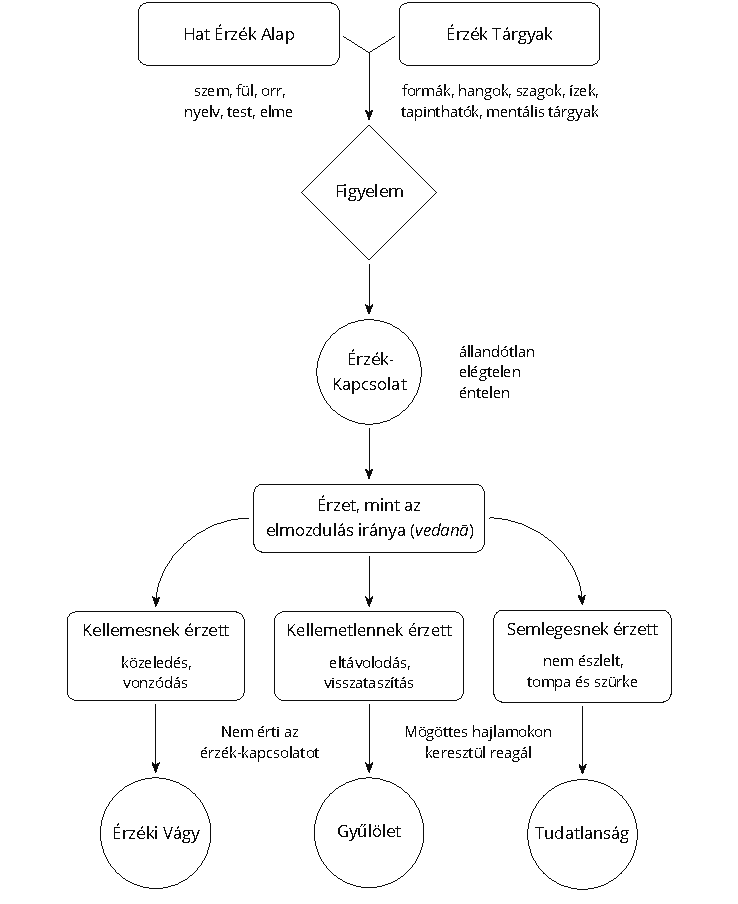
\includegraphics[width=\linewidth]{./manuscript/tex/diagrams/sense-contact-feeling-hu.pdf}
\end{figure}

\clearpage
\normalpagelayout

\vspace*{-\baselineskip}

\keywords{önnarratíva, elbeszélés}

Milyen hatással van ez arra, ahogy elbeszéljük magunknak a
tapasztalatainkat? Azt mondjuk magunknak, hogy ez az érzés jó volt vagy
rossz, és mit kellene erről gondolnunk. Egy központi eleme ennek a
narrátori szövegnek a \emph{mi érzéseink}, jellemzően abban az irányban,
hogyan legyen több a jó fajtából.

Mi történik, mikor észrevesszük, hogy mind a jó és a rossz tapasztalatok
instabilak, megbízhatatlanok, és a keletkezésük és elmúlásuk nincs az
irányításunk alatt? A belső értékeink átrendeződnek,
a vágy helyett a mulandóság által vezérelve.

\keywords{változékony természet, bölcs vizsgálódás}

Rendszerint akkor kezdünk csak figyelni, amikor észrevesszük, hogy
valami rossz, valami fáj, valami miatt szenvedünk. A kellemes
tapasztalatokra nem igénylünk annyi magyarázatot, ugye? Ezt a frusztrált
érzést, elégtelenséget és terjengő gondolkodást jelként használhatjuk a
magunk számára, hogy kezdjünk éberen vizsgálódni.

Gondolatban lépj egyet vissza, és figyeld a tapasztalatot mint egy
folyamatot, aminek van eleje, változáson megy keresztül, és megszűnik.
`A testben hol érzem ezt az érzést? Emlékszem, mikor kezdődött? Tudom
figyelni, ahogy változik? El tudom kapni, ahogy az érzés megszűnik?'

Nem tudjuk irányítani a világot magunk körül, de a hozzáállásunk
befolyásolja, mit látunk szabad választásként. A szemléletünk nyitja meg
vagy zárja be az ajtókat a tettek felé, amiket lehetségesnek látunk.
Ezek a tettek hozzák létre a helyzetet, amiben élünk, és befolyásolják,
ahogy a helyzetben látjuk magunkat. Ha nem vizsgáljuk a tapasztalataink
természetét, hajlamosak vagyunk a jó érzéseket jutalomnak és a rossz
érzéseket büntetésnek tekinteni, ennek folytán az életünk értelme ezek
körül fog forogni. A belső világunk mindig azokról a kérdésekről fog
szólni, mint: `Ki vagyok én \ldots{} Hogyan tegyem \ldots{} Miért kell
tegyem \ldots{} Mit kellene tennem \ldots{}' Nem olyan terhes érzés ez,
amit jobb lenne elhagyni?

Az alapos és felületes vizsgálat a \emph{szuttákban}\footnote{\href{https://a-buddha-ujja.hu/mn-2/hu/forizs-laszlo}{MN
  2}, Az összes káros folyamatról szóló tanítóbeszéd} használt
kifejezés, mely különbséget tesz a felületes figyelem között ami növeli
a zavarodottságunkat, és az alapos figyelem között ami tisztánlátáshoz
és helyes megértéshez vezet. A felületes vizsgálat átsiklik az
állandótlanság, elégtelenség és nem-én jellemzői felett, így mindent a
saját ügyének tekint. Az alapos vizsgálat felismeri az érzéki
tapasztalat jellemzőit, és a Négy Nemes Igazsággal összhangban
elmélkedik róluk.

\keywords{ragaszkodás az énhez, karóhoz kötött kutya, vizsgálódás}

Emlékszel, hogy egy kutya, pórázzal kikötve egy karóhoz, hogy futkos
körbe-körbe a karó körül? Ül, áll, járkál vagy futkos körülötte, de
minden amit tesz, a karó körül teszi.\footnote{\href{https://suttacentral.net/sn22.100}{SN
  22.100}, Póráz} Az ego által vezérelt gondolatok kavargása is ilyen.
Lehet, hogy elfoglaltan tart minket, de továbbra is ragaszkodunk a
középen lévő énhez, nem vagyunk képesek sehova máshova menni. A póráz az
azonosulás és megragadás (\emph{upādāna}), az a folyamat, ami kialakítja
az `én és enyém' képzetét az érzékek tapasztalatában, vagy akörül,
melynek alapvető igazság szerint nincs semmi ilyen jellemzője. Ez vezet
minket a felületes vizsgálathoz, arra összpontosítva kik vagyunk, mi
lesz velünk, növelve a kétségünket és zavarodottságunkat.

Az `én és enyém'-ben gyökerező kérdések csapdák. Egyre tovább
húznak-vonnak minket anélkül, hogy szabadsághoz vagy megálláshoz
vezetnének. Ha azt vesszük észre, hogy ki vagyunk kötve egy karóhoz, mit
tegyünk? Elvágni a pórázt jó ötletnek tűnik.

A meditáción belül értelmezve, a vizsgálódásra nem mindenféle
gondolkodás alkalmas. Nem minden fajta gondolat fog belátást
eredményezni. Vizsgálódó meditáció közben, a tapasztalatunkat ok-okozati
folyamatra bontjuk le, amire a Négy Nemes Igazságot\footnote{\href{https://a-buddha-ujja.hu/sn-56.11/hu/farkas-pal}{SN
  56.11}, A Tan kerekét forgásba hozó tanítóbeszéd} használjuk
útmutatóként.

Ez egy olyan tapasztalattal kezdődik, amit személyesen könnyű
azonosítanunk: a szenvedés, feszültség, elégtelenség, avagy Páli szóval
\emph{dukkha}. A gondolat iránya nem \emph{az én szenvedésem}, mint
személyes történet, hanem személytelen, természetes folyamatként
szemléljük azt.

\keywords{dukkha}

A kezdő álláspont azt elismerni, hogy a feszültség, a szenvedés
\emph{itt} van. Ez ismeretként triviális, hogy igen, van a világban
feszültség és szenvedés. De amikor magunk tapasztaljuk, szeretünk mégis
inkább valami másra figyelni, vagy hajlamosak vagyunk valakit hibáztatni
érte. Ezerféle dolgot teszünk, csak ne kelljen tudatosan elismerjük és
érdemben foglalkoznunk vele.

Az utasítás itt az, hogy csak az fog előre vezetni, ha a szenvedés felé
fordulunk, és azt vizsgálva keressük a megértés módját. A Buddha
tanításában ez az Első Nemes Igazság: van szenvedés, és a nemes
hozzáállás az, ha felé fordulunk és megértjük.

Mit értünk meg? Azt, hogy a szenvedés nem a semmiből jött létre, hanem
korábbi tényezők eredménye. Ha így tudjuk vizsgálni a helyzetet, nem
vagyunk tehetetlenek. Még ha nem is értjük a helyzetünk minden apró
tényezőjét, már az is megkönnyebbülés, hogy talán tudunk valamit
változtatni.

\keywords{a dukkha eredete}

A Második Nemes igazság arra mutat rá, hogy a szenvedést kiváltó okot
magunkban találjuk. Ez a kívánságunk, hogy a tapasztalataink másképpen
legyenek mint ahogy természetüktől fogva vannak. A görcsös
ragaszkodásunk ahhoz, ami állandótlan, törékeny, és nem megtartható. A
szenvedés, a \emph{dukkha} amit tapasztalunk, ettől a ragaszkodástól,
szomjas vágytól függ. Az utasítás, a nemes hozzáállás itt az, hogy ezt a
szomjas vágyat és ragaszkodást el kell engednünk, mert a mulandó
élményekhez való ragaszkodás szenvedés.

\keywords{a dukkha megszűnése}

A kiváltó ok megszűnésével megszűnik az eredmény, a szenvedés is. A jó
hír, hogy a szenvedés végét is magunkban találjuk.

Ebből a szemszögből láthatjuk, hogy az elme hozza létre azt a fajta
világot, amiben élünk. Ha figyeljük, van esélyünk, hogy legalább ne
rontsunk a helyzeten. És ki tudja, akár még javíthatunk is rajta?

A Harmadik Nemes Igazság erre irányítja a figyelmünket: van megoldás,
nem kötelező keserűségben és értelmetlen küszködésben élnünk. A tanács,
a nemes hozzáállás az, hogy gyakoroljunk és tapasztaljuk ezt meg a
magunk számára, a megértésen és a ragaszkodás elengedésén keresztül. Így
lehetővé tesszük a szenvedés megszűnését.

\clearpage

Még ha nem is tudjuk rögtön elengedni, már az is megkönnyebbülés, ha
látjuk az összefüggést: `Ha elengedném, nem szenvednék tőle'.
Ez már a munka fele. Egész eddig térkép nélkül bolyongtunk, de innen már
van út előre.

\keywords{a gyakorlás útja}

A Negyedik Nemes Igazság az út gyakorlását írja le. A Buddha nyolc
tényezőre bontotta, melyek magukban foglalják a mindennapi élet
helyzeteit és a meditáció fejlesztését is.

A Nyolcrétű Ösvény részei a (1) megértés, (2) szándék, (3) beszéd, (4)
tett, (5) megélhetés, (6) erőfeszítés, (7) éberség és (8) elmélyülés.
Amikor egy tényező összhangban van az igazsággal, \emph{helyesnek}
nevezzük: Helyes Megértés, Helyes Szándék, és így tovább. Az utat
részekre bontani segíti a vizsgálódást, könnyebb ilyen módon
gondolkodnunk, de az út tényezői nem különállóak: egymást erősítik és
támogatják. A gyakorlás egyesült egészként valósul meg.

Amikor leginkább szükségünk van a gyakorlásra, az \emph{azonnal} kell.
Nem állhatunk meg tényezőket számolni. Olyan eszköz hasznos, ami
hordozható és könnyen elérhető egy adott helyzetben. Mikor olvasunk,
töprengünk a jelentésen, van időnk körbejárni a szavakat, ez a tanulás
szakasza. Viszont az éber figyelem, mint elvont ötlet nem sokat használ
-- akkor értékes, ha gyakoroljuk, mikor kéznél van a jelen pillanatban.

\enlargethispage*{\baselineskip}

Mindig ide térünk vissza. Emlékszünk a múltra és tervezzük a jövőt, de
az emlékezés egy jelen tapasztalat, a tervezés egy jelen tapasztalat. A
meditáció gyakorlását nem a jövőért végezzük. Ha a megértést,
szabadságot, boldogságot, akadályok túllépését egy jövőbeli állapotként
látjuk, ezzel csak több lesz a terhünk. Az elengedés a jelenben
történik, ahol az állapotok nélkülünk változnak.
